\section{CLIQUES Algorithm}
In our research, we will use the idea of the clique to extract the candidate of descriptive patterns, to be exact, bipartite clique. In the mathematical field of graph theory, a clique is a subset of the vertices of an undirected graph, so that each of the two vertices of the subgraph is adjacent to each other, that is, its induced subgraph is complete. Cliques are one of the basic concepts of graph theory. They are also widely used in many other mathematical problems and graph theory, it is also very popular in computer science: the task of finding whether there is a clique of a given size is NP-complete. But although the hardness results for many factions, many algorithms have been studied. What we talk here is one of them called CLIQUES, developed by Etsuji Tomita, Akira Tanaka, and Haruhisa Takahashi, from The University of Electro-communications. We can find maximal cliques from a graph by CLIQUES Algorithm, we will talk about how to do with the bipartite graph, and find bipartite cliques.\\
In the mathematical field of graph theory, a bipartite graph is a graph where the vertex in it can be divided into two disjoint sets $U$ and $V$, $U$ and $V$ are each independent sets. And every edge connects one vertex in $U$ and one vertex in $V$. Bipartite Clique is a special subgraph of a bipartite graph, where each pairs from vertex set $U$ and vertex set $V$  are connected. If we connect all vertex form $U$ with each other and do the same process to set $V$, we can find a bipartite clique becomes a normal clique. Conversely, if we want to find bipartite cliques in a bipartite graph, we can connect all vertexes from the same set, and make it be a normal graph, the vertexes in clique also form bipartite clique as a subgraph of the original bipartite graph. We will introduce CLIQUES Algorithm which can extract all maximal cliques form a graph very fast.\\
CLIQUES is a depth-first algorithm for generating all maximal cliques of an undirected graph, in which pruning methods are employed as in the B-K algorithm[8]. All of the results, which are maximal cliques are produced in a tree-like form. And its worst-case time complexity is $O(3^{n/3})$ for an n-vertex graph.[6] \\
We are concerned a simple undirected graph $G=(V,E)$ with a finite set $V$ of verices and a finite set $E$ of unordered pairs $(v,w)$ of idstinct vertices, we call them edges. We also call the pair of vertices $v$ and $w$ adjacent if $(v,w)\in E$. For any vertex $v\in V$, we call $\mathcal{T}(v)$ is the set of verties that are adjacent to $v$ in $G = (V,E)$, For example, $\mathcal{T}(V) = \{w\in V | (v,w)\in E\}$. For a subset $W \subseteq V$ of vertices, $G(W) = (W,E(W))$ with $E(W)=\{(v,w)\in W \times W|(v,w)\in E\}$ is called a subgraph of $G = (V,E)$ induced by $W$. For a set $W$ of vertices, $|W|$ donotes the number of elements in $W$. Given a subset $W \subseteq V$ of vertices, the induced subgraph $G(Q)$ is called to be complete if $(v,w)\in E$ for all of vertices $v,w \in Q$ with $v \ne w$. In this situation, we can simply state that $Q$ is a complete subgraph. We call a complete subgraph a clique. We call a clique a maximal clique if the clique is not a proper subgraph of any other cliques. After understand the basic knowledge about clique, we can start our algorithm.[6]\\ \\
\textbf{CLIQUES}
\\ \\
We have mentioned before, CLIQUES is a depth-first algorithm for generating all maximal clique of a give undirected graph $G=(V,E)\ V\ne \emptyset$.\\
For the processing of algorithm, we have a global variable $Q$ of a set of vertices that constructs a complete subgraph, clique, found up. THe algorithm starts with set $Q$ as an expty set, and expands $Q$ step by step over applying the recuresive procedure $EXPAND$ to $V$ and its goal induced subgraphs to search for all complete subgraphs until they become maximal subgraphs.\\
Let $Q = \{p_1,p_2,...p_j\}$ become a complete subgraph found over some processing, and consider the vertices:
\begin{displaymath}
SUBG = C \cap \mathcal{T}(p_1)\cap \mathcal{T}(p_2)\cap ... \cap\mathcal{T}(p_j)
\end{displaymath}
where $SUBG=V$ and $Q = \emptyset$ as the initialization. We apple $EXPAND$ to $SUBG$ for searching for a larger complete subgraph. If we meet the situation of $SUBG = \emptyset$, we can say $Q$ is a maximal complete subgraph, or a maximal clique. Else, $Q\cup{q}$ will be a larger complete subgraph for every $q\in SUBG$. In this case, we consider a smaller subgraph set $G(SUBG_q)$ in which the graphs are induced by new set of vertices:
\begin{displaymath}
SUBG_q = SUBG \cap \mathcal{T}(q)
\end{displaymath}
for all $q \in SUBG$; we will also apply $EXPAND$ to $SUBG_q$ for finding larger complete subgraphs containing $Q\cup{q}$.\\
So far, we have only described the well-known basic framework of generating algorithms for all the maximal complete subgraphs, maximal cliques. This process can be represented by the following search or collection of search trees: The root set of the search forest is exactly the same as the $V$ of the graph $G = (V, E)$. For each $q \in SUBG$, all vertices in $SUBG_q$ are children of q. Thus, a set of vertices along the path from the root to any vertex of the search tree form a complete subgraph or we can say a clique.\\
The most important point of CLIQUES Algorithm is pruning unnecessary parts. We have two methods, which are the same as the Brom-Kerbosch Algorithm.We treat the previously constructed $SUBG(\ne \emptyset)$ as an ordered set of vertices, and we continue to generate maximal cliques from the vertices in the SUBG in order.\\
First of all, $FINI$ will be the sebset of vertices of $SUBG$ which have benn processed by the algorithm. We use $CAND$ to represent the remaining sets of extended candidates: $CAND = SUBG-FINI$, So we have:
\begin{displaymath}
SUBG = FINI \cup CAND
\end{displaymath}
$FINI = \emptyset$ as the initialization. We will also have:
\begin{displaymath}
SUBG_q = FINI_q \cup CAND_q
\end{displaymath}
where,
\begin{displaymath}
FINI_q = FINI \cap \mathcal{T}(q) and CAND_q = CAND \cap \mathcal{T}(q)
\end{displaymath}
According to the processing, we can find that, only the vertices in $CAND_q$ will be the candidates for expanding the complete subgraph $Q\cup{q}$ for find a larger maximal complete subgraph. After that, all the cliques containing $(Q\cup{q})\cup{r}with r\in FINI_q \subseteq FINI$ will generate for any $r$ by the processing of procedure $EXPAND$ to $FINI$.\\
The second step, Given a vertex $u \in SUBG$, it is assumed that all the maximal cliques containing $Q \cup {u}$ have been generated. Then each new maximal clique containing $Q$ instead of $Q \cup {u}$ must contain at least one vertex $q \in SUBG - (u)$. This is because $R \cup {u}$ is a larger complete subgraph if $Q$ is extended to a complete subgraph $R = (Q\cup S) \cap (SUBG - {u})$ with $S \subseteq SUBG \cap (u)$ So $R$ is not a maximal one. Thus, by extending $Q$ to $Q \cup {q}$, any new largest group can be found such that $q \in SUBG - (u)$, and then all sets containing $Q \cup {q}$ are generated.\\
\newpage
From the following figure, we can easily understand the processing of CLIQUES Algorithm.
\begin{figure}[!hbp]
\centering
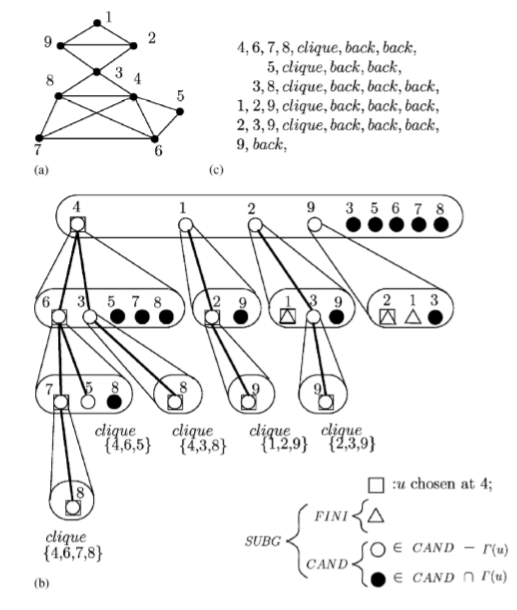
\includegraphics[width=400pt]{./pictures/0204.png}
\caption{an example of CLIQUES Algorithm}
\end{figure}
\newpage
In our research, we won't use any normal maximal, we will use the bipartite maximal cliques. To get bipartite maximal cliques from the bipartite graph using CLIQUES algorithm, we need some techniques. We have a figure to show it clearly.
\begin{figure}[!h]
\centering
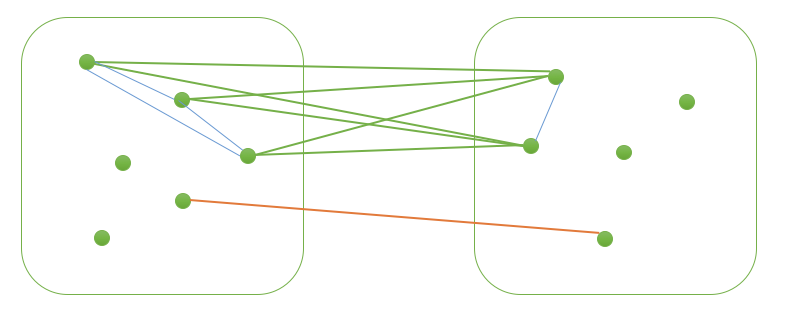
\includegraphics[width=350pt]{./pictures/0204-1.png}
\caption{bipartite clique}
\end{figure}
From the figure we can see that, the nodes connected by green link make a bipartite clique, if we also connect all the nodes in the same node set, the bipartite clique becomes a clique. So when we want to find maximal bipartite clique from a bipartite graph, we can connect all the nodes in the same node set, and make a normal graph[7], find the maximal clique in it, we can reconstruct all maximal bipartite clique from the clique result.